%==============================================================================
% presentation.tex
%==============================================================================


%==============================================================================
% Configuration
%==============================================================================

% Internationalisation
\usepackage[utf8]{inputenc}
\usepackage[T1]{fontenc}
% \usepackage[ngerman]{babel}

% Different packages
\usepackage{url}
\usepackage{color,listings,paralist}
\usepackage{enumerate}
\usepackage{tabularx}
\usepackage{alltt}

% Use default Acrobat reader fonts
\usepackage{mathpazo}

% Use CM fonts (increases document size)
\usepackage{ae}

% Use images
\usepackage{graphicx}

% Configure beamer
\usetheme[secheader]{Ikhono}
\usefonttheme[onlylarge]{structurebold}
\setbeamertemplate{navigation symbols}{}

% Variables
\providecommand{\Title}{Parallel Programming}
\providecommand{\Subtitle}{Recitation Session 7}
\providecommand{\Author}{Thomas Weibel <weibelt@ethz.ch>}
\providecommand{\Institute}{Laboratory for Software Technology, \\
  Swiss Federal Institute of Technology Z\"urich}
\providecommand{\Date}{April 22, 2010}

% PDF settings
\hypersetup{
  pdftitle={\Title, \Subtitle},
  pdfauthor={\Author},
  pdfsubject={\Institute},
  pdfkeywords={parallel programming} 
}

% Titlepage
\title{\Title}
\subtitle{\Subtitle}
\author{\Author}
\institute{\Institute}
\date{\Date}

% Listings
\lstdefinestyle{Default}{
  language=Java,
  tabsize=2,
  mathescape=true,
  inputencoding=utf8,
  showstringspaces=false,
  fontadjust=true,
  basicstyle=\ttfamily,
  keywordstyle=\color{blue}\bfseries,
}
\lstset{style=Default}


%==============================================================================
% Document
%==============================================================================

\begin{document}


% Titlepage
\begin{frame}[plain]
  \titlepage
\end{frame}


\section*{Introduction}

\begin{frame}{Executive Summary}
  \begin{itemize}
  \item Determining when a thread has finished
  \item The Volatile Returns
  \item Solution to the last assignment
  \item Semaphores
  \item Implementing Monitors with Semaphores
  \item \lstinline!wait()!, \lstinline!notify()!,
    \lstinline!notifyAll()!
  \item Hints for assignment 7
  \end{itemize}
\end{frame}


\section{Determining when a Thread has finished}

\begin{frame}{Outline}
  \tableofcontents[current]
\end{frame}

\begin{frame}[fragile]{\lstinline{isAlive()}}
\begin{lstlisting}
// Create and start a thread 
Thread thread = new MyThread(); 
thread.start(); 

// Check if the thread has finished 
// in a non-blocking way 
if (thread.isAlive()) { 
  // Thread has not finished 
} else { 
  // Finished 
} 
\end{lstlisting}
\end{frame}

\begin{frame}[fragile]{\lstinline{join(delayMillis)}}
\begin{lstlisting}
// Wait for the thread to finish but don't 
// wait longer than a specified time 
long delayMillis = 5000; // 5 seconds 
try { 
  thread.join(delayMillis); 
  if (thread.isAlive()) { 
    // Timeout occurred, 
    // thread has not finished 
  } else { 
    // Finished 
  } 
} catch (InterruptedException e) { 
  // Thread was interrupted 
} 
\end{lstlisting}
\end{frame}

\begin{frame}[fragile]{\lstinline{join()}}
\begin{lstlisting}
// Wait indefinitely for the thread to finish 
try { 
  thread.join(); 
  // Finished 
} catch (InterruptedException e) { 
  // Thread was interrupted 
} 
\end{lstlisting}
\end{frame}


\section{Volatile}

\begin{frame}{Outline}
  \tableofcontents[current]
\end{frame}

\begin{frame}{The Volatile Returns}
  \begin{itemize}
  \item Volatile variables are not cached in registers or in
    caches where they are hidden from other processors
  \item A read of a volatile variable always returns the most recent
    write by any thread
  \end{itemize}

  \vspace{\stretch{1}}
  
  \begin{center}
    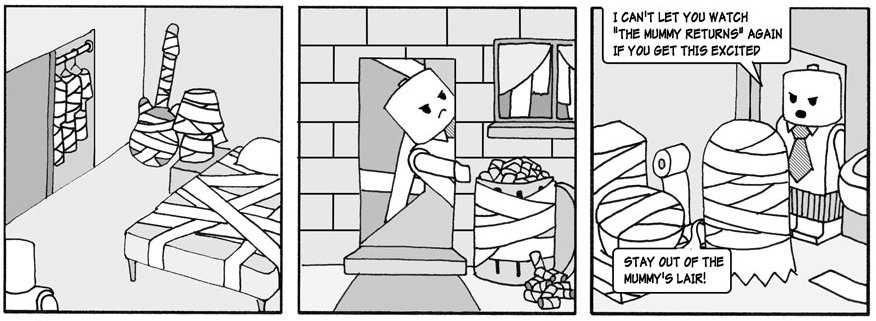
\includegraphics[width=\textwidth]{figures/the-mummy-returns} \\
    \tiny{Source: \url{http://thescope.ca/comics/everybodycheerup/the-mummy-returns}}
  \end{center}
\end{frame}

\begin{frame}[fragile]{Example}
\begin{lstlisting}[basicstyle=\fontsize{7}{9}\selectfont\ttfamily]
public class ShutdownDriver {
  boolean shutdown = false;

  public static void main(String[] args) throws InterruptedException {
    ShutdownDriver driver = new ShutdownDriver();
    new BusyTask(driver).start();
    Thread.sleep(2000);
    driver.shutdown = true;
  }
}

public class BusyTask extends Thread {
  private ShutdownDriver driver;

  public BusyTask(ShutdownDriver driver) {
    this.driver = driver;
  }

  public void run() {
    while (!driver.shutdown) {}
    System.out.println("Busy task stopped!");
  }
}
\end{lstlisting}
\end{frame}

\begin{frame}[fragile]{Example: Volatile}
\begin{lstlisting}[basicstyle=\fontsize{7}{9}\selectfont\ttfamily]
public class ShutdownDriver {
  volatile boolean shutdown = false;

  public static void main(String[] args) throws InterruptedException {
    ShutdownDriver driver = new ShutdownDriver();
    new BusyTask(driver).start();
    Thread.sleep(2000);
    driver.shutdown = true;
  }
}

public class BusyTask extends Thread {
  private ShutdownDriver driver;

  public BusyTask(ShutdownDriver driver) {
    this.driver = driver;
  }

  public void run() {
    while (!driver.shutdown) {}
    System.out.println("Busy task stopped!");
  }
}
\end{lstlisting}
\end{frame}

\begin{frame}{Synchronization}
  \begin{block}{Reading}
    Reading a volatile field is like acquiring a lock: The working
    memory is invalidated and the volatile field’s current value is
    reread from memory
  \end{block}

  \vspace{\stretch{1}}

  \begin{block}{Writing}
    Writing a volatile field is like releasing a lock: the volatile
    field is immediately written back to memory
  \end{block}
\end{frame}

\begin{frame}{Limitations}
  \begin{itemize}
  \item Although reading and writing a volatile field has the same
    effect on memory consistency as acquiring and releasing a lock,
    multiple reads and writes are not atomic
  \item For example, if \lstinline!x! is a volatile variable, the
    expression \lstinline!x++!  will not necessarily increment
    \lstinline!x! if concurrent threads can modify \lstinline!x!
  \item One common usage pattern for volatile variables occurs when a
    field is read by multiple threads, but only written by one
  \end{itemize}

  \vspace{\stretch{1}}

  \begin{alertblock}{No Atomicity!}
    \lstinline!volatile! alone is not strong enough to implement a
    counter, some form of mutual exclusion is needed as well
  \end{alertblock}
\end{frame}


\section{Last Assignment}

\begin{frame}{Outline}
  \tableofcontents[current]
\end{frame}

\begin{frame}[fragile]{Code}
  \begin{columns}[c]
    \begin{column}{0.50\textwidth}
\begin{lstlisting}[basicstyle=\fontsize{9}{11}\selectfont\ttfamily]
A1 // non-critical section
A2 turn0.flag = 0;
A3 while(true)
     if(turn1.flag == 1) 
       break;
A4   turn0.flag = 1;
A5   turn0.flag = 0;
   }
A6 // critical section
A7 turn0.flag = 1;
\end{lstlisting}
    \end{column}
    \begin{column}{0.50\textwidth}
\begin{lstlisting}[basicstyle=\fontsize{9}{11}\selectfont\ttfamily]
B1 // non-critical section
B2 turn1.flag = 0;
B3 while(true) {
     if(turn0.flag == 1) 
       break;
B4   turn1.flag = 1;
B5   turn1.flag = 0;
   }
B6 // critical section
B7 turn1.flag = 1;
\end{lstlisting}
    \end{column}
  \end{columns}
\end{frame}

\begin{frame}[fragile]{Invariants}
  \begin{enumerate}
  \item \lstinline!at(A6)! $\rightarrow$ \lstinline!turn0.flag == 0!
  \item \lstinline!at(B6)! $\rightarrow$ \lstinline!turn1.flag == 0!
  \item \lstinline!not [at(A6) AND at(B6)]!
  \end{enumerate}

  \vspace{\stretch{1}}

  We use the notation ``\lstinline!at(S)!'' to indicate that execution
  is ``at statement (location) \lstinline!S!'' $\Rightarrow$ all
  previous statements have executed while \lstinline!S! has not yet
  started to execute
\end{frame}

\begin{frame}[fragile]{Proof (1)}
  \begin{itemize}
  \item \lstinline!at(A1)!, \lstinline!at(A2)!, \lstinline!at(A3)!,
    \lstinline!at(A4)!, \lstinline!at(A5)!, \lstinline!at(A7)!: 
    antecedent \lstinline!at(A6)! is false
  \item \lstinline!at(A6)!:
    \begin{itemize}
    \item can only get to \lstinline!A6! via \lstinline!A3!;
    \item can only get to \lstinline!A3! via \lstinline!A2!;
    \item \lstinline!A2! sets \lstinline!turn0.flag! to \lstinline!0!
    \end{itemize}
  \item Thread \lstinline!B! does not modify \lstinline!turn0!
  \end{itemize}
\end{frame}

\begin{frame}[fragile]{Proof (2)}
  Same way. Please do it if you had trouble with proof of (1).
\end{frame}

\begin{frame}[fragile]{Proof (3): By Contradiction}
  \begin{itemize}
  \item Assume thread \lstinline!A! is at state \lstinline!A6!:
    \begin{itemize}
    \item Hence \lstinline!turn0.flag == 0! (invariant (i))
    \item After some time, thread \lstinline!B! wants to enter
      \lstinline!B6!, which would require \lstinline!turn0.flag == 1!
    \end{itemize}
  \item Contradiction: \lstinline!turn0.flag! cannot be \lstinline!0!
    and \lstinline!1! at the same time
  \item Equivalent proof for thread \lstinline!B!
  \end{itemize}
\end{frame}


\section{Review of Semaphores}

\begin{frame}{Outline}
  \tableofcontents[current]
\end{frame}

\begin{frame}{Semaphores}
  \begin{columns}[c]
    \begin{column}{0.50\textwidth}
      \begin{itemize}
      \item Special integer variable with two atomic operations
        \begin{itemize}
        \item \lstinline!P()!: Passeren, wait/up
        \item \lstinline!V()!: Vrijgeven/Verhogen, signal/down
        \end{itemize}
      \item Names of operations reflect the Dutch origin of the
        inventor...
      \end{itemize}
    \end{column}
    \begin{column}{0.50\textwidth}
      \begin{center}
        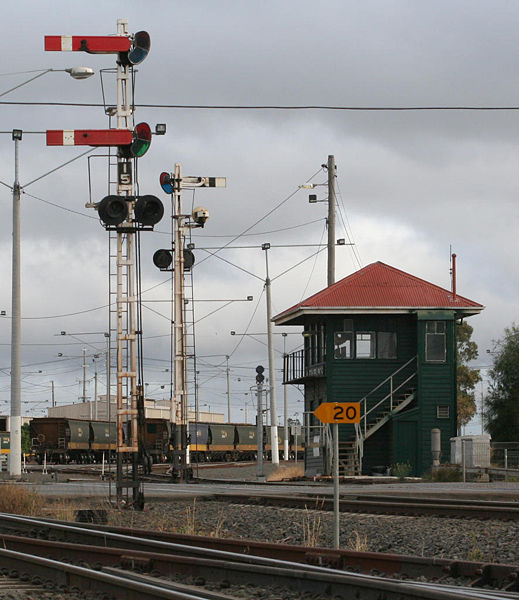
\includegraphics[width=\textwidth]{figures/semaphores} \\
        \tiny{Source: \url{http://en.wikipedia.org/wiki/File:Mechanical-signalling-north-geelong.jpg}}
      \end{center}
    \end{column}
  \end{columns}
\end{frame}

\begin{frame}[fragile]{Class \lstinline!Semaphore!}
\begin{lstlisting}
public class Semaphore {
  private int value;
  public Semaphore() { 
    value = 0; 
  }
  public Semaphore(int k) { 
    value = k; 
  }
  public synchronized void P() { 
    /* see later */ 
  }
  public synchronized void V() { 
    /* see later */ 
  }   
}
\end{lstlisting}
\end{frame}

\begin{frame}[fragile]{\lstinline!P()! Operation}
\begin{lstlisting}
public synchronized void P() {
  while (value == 0) {
    try {
      wait();
    }
    catch (InterruptedException e) { 
    }
  }
  value--;
}
\end{lstlisting}
\end{frame}

\begin{frame}[fragile]{\lstinline!V()! Operation}
\begin{lstlisting}
public synchronized void V() {
  ++value;
  notifyAll();
}
\end{lstlisting}
\end{frame}

\begin{frame}{\lstinline!wait()!, \lstinline!notify()!, \lstinline!notifyAll()!}
  \begin{columns}[c]
    \begin{column}{0.5\textwidth}
      \begin{itemize}
      \item \lstinline!wait()! tells the calling thread to give up the
        monitor and go to sleep until some other thread enters the
        same monitor and calls \lstinline!notify()!
      \item \lstinline!notify()! wakes up the first thread that called
        \lstinline!wait()! on the same object
      \item \lstinline!notifyAll()! wakes up all the threads that
        called \lstinline!wait()! on the same object, the highest
        priority thread will run first
      \end{itemize}
    \end{column}
    \begin{column}{0.5\textwidth}
      \begin{center}
        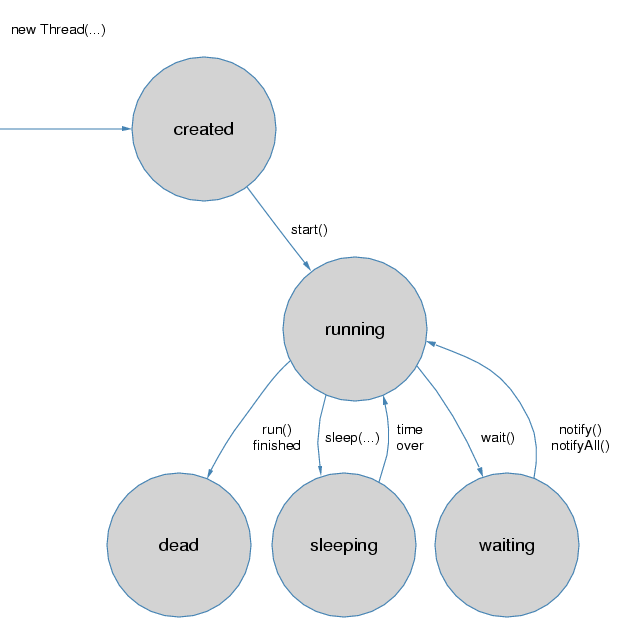
\includegraphics[width=\textwidth]{figures/thread}
      \end{center}
    \end{column}
  \end{columns}
\end{frame}

\begin{frame}{Comments}
  \begin{itemize}
  \item You can only modify the value of a semaphore instance using
    the \lstinline!P()! and \lstinline!V()! operations.
    \begin{itemize}
    \item Initialize in constructor
    \end{itemize}
  \item Effect
    \begin{itemize}
    \item \lstinline!P()! may block 
    \item \lstinline!V()! never blocks
    \end{itemize}
  \item Application of semaphores:
    \begin{itemize}
    \item Mutual exclusion
    \item Conditional synchronization
    \end{itemize}
  \end{itemize}
\end{frame}

\begin{frame}[fragile]{Semaphores}
  \begin{itemize}
  \item Binary  semaphore
    \begin{itemize}
    \item Value is either 0 or 1
    \item Supports implemention of  mutual exclusion:
\begin{lstlisting}
Semaphore s = new Semaphore(1);
s.P()
//critical section
s.V()
\end{lstlisting}
    \end{itemize}
  \item Counting (general) semaphore
    \begin{itemize}
    \item Value can be any positive integer value
    \end{itemize}
  \end{itemize}
\end{frame}

\begin{frame}{Fairness}
  \begin{itemize}
  \item A semaphore is considered to be ``fair'' if all threads that
    execute a \lstinline!P()! operation eventually succeed
  \item Semaphore is ``unfair'': a thread blocked in the
    \lstinline!P()! operation must wait forever while other threads
    (that executed the operation later) succeed.
  \end{itemize}

  \vspace{\stretch{1}}
  
  \begin{center}
    
\includegraphics[scale=0.4]{figures/dilbert-fairness}
  \end{center}
\end{frame}

\begin{frame}{Semaphores in Java}
  \begin{itemize}
  \item \lstinline!java.util.concurrent.Semaphore!
    \begin{itemize}
    \item \lstinline!acquire()! instead of \lstinline!P()!
    \item \lstinline!release()! instead of \lstinline!V()!
    \end{itemize}
  \item Constructors
    \begin{itemize}
    \item \lstinline!Semaphore(int permits)!
    \item \lstinline!Semaphore(int permits, boolean fair)!
      \begin{itemize}
      \item \lstinline!permits!: initial value
      \item \lstinline!fair!: if true then the semphore uses a FIFO to
        manage blocked threads
      \end{itemize}
    \end{itemize}
  \end{itemize}
\end{frame}


\section{Semaphore Implementation of Monitors}

\begin{frame}{Outline}
  \tableofcontents[current]
\end{frame}

\begin{frame}{Semaphores and Monitors}
  \begin{itemize}
  \item Monitor: model for synchronized methods in Java
  \item Both constructs are equivalent
  \item One can be used to implement the other
  \end{itemize}

  \vspace{\stretch{1}}
  
  \begin{center}
    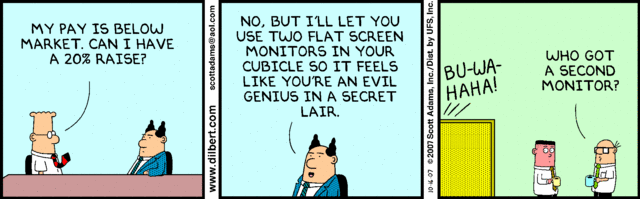
\includegraphics[scale=0.4]{figures/dilbert-monitor}
  \end{center}
\end{frame}

\begin{frame}{Example}
  See slides from March 18 for context
\end{frame}

\begin{frame}[fragile]{Buffer using condition queues}
\begin{lstlisting}[basicstyle=\fontsize{9}{11}\selectfont\ttfamily]
class BoundedBuffer extends Buffer {
  public BoundedBuffer(int size) { 
    super(size);
  }
  public synchronized void insert(Object o) 
    throws InterruptedException {
    while (isFull())
      wait();
    doInsert(o);	
    notifyAll();
  }
  public synchronized Object extract() 
    throws InterruptedException {
    while (isEmpty())
      wait();
    Object o = doExtract();
    notifyAll();
    return o;
  }
}
\end{lstlisting}
\end{frame}

\begin{frame}{Emulation of monitor with semaphores}
  We need 2 semaphores:
  \begin{itemize}
  \item	One to make sure that only one synchronized method executes at any given time
    \begin{itemize}
    \item call this the ``access semaphore'' \lstinline!S!
    \item binary semaphore
    \end{itemize}
  \item One semaphore to line up threads that are waiting for some condition
    \begin{itemize}
    \item call this the ``condition semaphore'' \lstinline!SCond!
    \item binary semaphore
    \item threads that wait must do an ``acquire''
    \end{itemize}
  \end{itemize}

  \vspace{\stretch{1}}

  \begin{block}{For convenience}
    Counter \lstinline!waitThread! to count number of waiting threads
    i.e., threads in queue for \lstinline!SCond!
  \end{block}
\end{frame}

\begin{frame}{Basic idea}
  \begin{enumerate}
  \item Frame all synchronized methods with \lstinline!S.acquire()! and
    \lstinline!S.release()!
    \begin{itemize}
    \item This ensures that only one thread executes a synchronized
      method at any point in time
    \item Recall: \lstinline!S! is binary.
    \end{itemize}
  \item Translate \lstinline!wait()! and \lstinline!notifyAll()! to give threads waiting in
    line a chance to progress (these threads use \lstinline!SCond!)
    \begin{itemize}
    \item To simplify the implementation, we require that
      \lstinline!notifyAll()! is the last action in a synchronized
      method
    \item Java does not enforce this requirement but the mapping of
      synchronized methods into semaphores is simplified
    \end{itemize}
  \end{enumerate}
\end{frame}

\begin{frame}[fragile]{Buffer with auxiliary fields}
\begin{lstlisting}
class BoundedBuffer extends Buffer {
  public BoundedBuffer(int size) { 
    super(size);
    access = new Semaphore(1);
    cond = new Semaphore(0);
  }

  private Semaphore access;
  private Semaphore cond;
  private int waitThread = 0;
  
  // continued
\end{lstlisting}
\end{frame}

\begin{frame}[fragile]{(1) Framing all methods}
\begin{lstlisting}
public void insert(Object o)
  throws InterruptedException {
  access.acquire(); // ensure mutual exclusion

  while (isFull())
    wait();

  doInsert(o);	
  notifyAll();

  access.release();
}
\end{lstlisting}
\end{frame}

\begin{frame}{Notes}
  \begin{itemize}
  \item There is one semaphore for all synchronized methods of one
    instance of \lstinline!BoundedBuffer!:
    \begin{itemize}
    \item Must make sure that insert and extract don't overlap
    \end{itemize}
  \item There must be separate semaphore to deal with waiting
    threads:
    \begin{itemize}
    \item Imagine the buffer is full. A thread that attempts to insert
      an item must wait. But it must release the access
      semaphore. Otherwise a thread that wants to remove an item will
      not be able to executed the (synchronized!) extract method.
    \end{itemize}
  \end{itemize}
\end{frame}

\begin{frame}[fragile]{(2) Translate \lstinline!wait()!}
\begin{lstlisting}
waitThread++;

// other threads can execute 
// synchronized methods 
S.release(); 

// wait till condition changes
SCond.acquire(); 
S.acquire();

waitThread--;
\end{lstlisting}
\end{frame}

\begin{frame}[fragile]{(2) Translate \lstinline!notifyAll()!}
\begin{lstlisting}
if (waitThread > 0) {
  for (int i=0; i < waitThread; i++) { 
    SCond.release();
  }
}	
\end{lstlisting}

  \vspace{\stretch{1}}

  \begin{itemize}
  \item All threads waiting are released and will compete to
    (re)acquire \lstinline!S!
  \item They decrement \lstinline!waitThread! after they leave
    \lstinline!SCond.acquire()!
  \item Note that to enter the line (i.e., increment
    \lstinline!waitThread!) the thread must hold the access semaphore
    \lstinline!S!
  \end{itemize}
\end{frame}

\begin{frame}{(2) Translate \lstinline!wait()! and \lstinline!notifyAll()!}
  \begin{itemize}
  \item Recall that \lstinline!S.release()! is done at the end of the
    synchronized method
  \item So all the threads that had lined up waiting for
    \lstinline!SCond! compete to get access to \lstinline!S!
  \item No thread can line up while the \lstinline!SCond.release()!
    operations are done since this thread holds \lstinline!S!
  \end{itemize}
\end{frame}

\begin{frame}{Note}
  \begin{itemize}
  \item We wake up all threads -- they might not be able to enter
    their critical section if the condition they waited for does not
    hold, but all threads get a chance.
  \item This approach is different from what we discussed in the
    lecture
  \end{itemize}
\end{frame}

\begin{frame}[fragile]{Translate \lstinline!wait()!}
\begin{lstlisting}[basicstyle=\fontsize{9}{11}\selectfont\ttfamily]
public void insert(Object o)
  throws InterruptedException {
  access.acquire();
  while (isFull()) {
    waitThread++;
    access.release(); // let other thread access object
    cond.acquire(); // wait for change of state
    access.acquire()
    waitThread--;
  }
  doInsert(o);	
  notifyAll();
  access.release();
}
\end{lstlisting}
\end{frame}

\begin{frame}[fragile]{Translate \lstinline!notifyAll()!}
\begin{lstlisting}[basicstyle=\fontsize{9}{11}\selectfont\ttfamily]
public void insert(Object o) 
  throws InterruptedException {
  access.acquire();
  while (isFull()) {
    waitThread++;
    access.release(); // let other thread access object
    cond.acquire(); // wait for change of state
    access.acquire()
    waitThread--;
  }
  doInsert(o);	
  if (waitThread > 0) { 
    for (int i; i < waitThread; i++) {
      cond.release(); 
    } 
  }
  access.release(); 
}
\end{lstlisting}
\end{frame}

\begin{frame}{Example}
  Consider the buffer, one slot is empty, four operations

  \vspace{\stretch{1}}

  \begin{enumerate}
  \item \lstinline!insert I1!
  \item \lstinline!insert I2!
  \item \lstinline!insert I3!
  \item \lstinline!extract E!
  \end{enumerate}
\end{frame}

\begin{frame}{Example}
  \begin{itemize}
  \item \lstinline!I1! -- \lstinline!access.acquire()!
  \item \lstinline!I2! -- \lstinline!access.acquire()!: blocks on
    access
  \item \lstinline!I3! -- \lstinline!access.acquire()!: blocks on
    access
  \item \lstinline!I1! -- \lstinline!waitThread == 0!
  \item \lstinline!I1.release!
  \item \lstinline!I2! -- \lstinline!access.acquire()! completes
  \item \lstinline!I2! -- buffer full
  \item \lstinline!waitThread = 1!
  \item \lstinline!I2! -- \lstinline!access.release()!
  \item \lstinline!I2! -- \lstinline!cond.acquire()! -- blocks on \lstinline!cond!
  \item \lstinline!I3! -- \lstinline!access.acquire()! completes
  \item \lstinline!I3! -- buffer full
  \end{itemize}
\end{frame}

\begin{frame}{Example}
  \begin{itemize}
  \item \lstinline!waitThread = 2!
  \item \lstinline!I3! -- \lstinline!access.release()!
  \item \lstinline!I3! -- \lstinline!cond.acquire! -- blocks on \lstinline!cond!
  \item \lstinline!E! -- \lstinline!access.acquire()!
  \item remove item
  \item \lstinline!E! -- \lstinline!SCond.release()!
  \item \lstinline!E! -- \lstinline!SCond.release()!
  \item \lstinline!E! -- \lstinline!access.release()!
  \end{itemize}

  \vspace{\stretch{1}}

  One of \lstinline!I2! or \lstinline!I3! will succeed with
  \lstinline!access.acquire()! and be able to insert the next item
\end{frame}

\begin{frame}{Exercise}
  How would the method \lstinline!extract! look like if we used
  semaphores to emulate monitors?
\end{frame}


\section{Assignment 7}

\begin{frame}{Outline}
  \tableofcontents[current]
\end{frame}

\begin{frame}{Read/Write Lock}
  \begin{itemize}
  \item Many shared objects have the property that most method calls
    return information about the object's state without modifying the
    object ({\bf readers}) while only a small number of calls actually
    modify the object ({\bf writers})
  \item There is no need for readers to synchronize with one another
    \begin{itemize}
    \item It is perfectly safe for them to access the object
      concurrently
    \end{itemize}
  \item Writers, on the other hand, must lock out readers as well as
    other writers
  \item A Read/Write Lock allows multiple readers or a single
    writer to enter the critical section concurrently
  \end{itemize}
\end{frame}

\begin{frame}{Overview}
  \begin{itemize}
  \item Your task is to implement a Read/Write Lock
  \item At most four threads
  \item At most two reader threads (shared access is allowed) and one
    writer thread
  \item A thread that executes \lstinline!read()! is a reader
    \begin{itemize}
    \item At a later time it can be a writer...
    \end{itemize}
  \end{itemize}
\end{frame}

\begin{frame}{Challenges}
  \begin{itemize}
  \item No starvation
  \item Efficient implementation
    \begin{itemize}
    \item If there are fewer than two readers and no waiting writers
      then the next reader must be allowed to proceed
    \item If there is no contention then a thread must be allowed to
      proceed immediately
    \end{itemize}
  \item Your implementation must be fair:
    \begin{itemize}
    \item You may want to use \lstinline!FIFOQueue.java! (part of the
      skeleton)
    \end{itemize}
  \end{itemize}
\end{frame}

\begin{frame}{Comments}
  \begin{itemize}
  \item Keep your solution as simple as possible
  \item Decide what you want to use:
    \begin{itemize}
    \item Monitors (synchronized methods)
    \item Semaphores \\
      (see \url{http://java.sun.com/javase/6/docs/api/})
    \end{itemize}
  \item Only change class \lstinline!Monitor.java! (part of the
    skeleton)
    \begin{itemize}
    \item If you feel it‘s necessary to change other files, please let
      us know
    \end{itemize}
  \item Please comment your code!
  \end{itemize}
\end{frame}

\begin{frame}{Hints}
  \begin{itemize}
  \item \lstinline!Thread.currentThread()! returns a handle to the
    current thread and might be useful for the assignment.
  \item \lstinline!Thread.currentThread().getId()!:
    \begin{itemize}
    \item \lstinline!waitList.enq(Thread.currentThread().getId())!
    \item \lstinline!waitList.getFirstItem() == !\\
      \lstinline!Thread.currentThread().getId()!
    \end{itemize}
  \end{itemize}
\end{frame}


\section*{Outro}

\begin{frame}{Summary}
  \begin{columns}[c]
    \begin{column}{0.50\textwidth}
      \begin{itemize}
      \item Different ways to determine if a thread finished
      \item Volatile
      \item Semaphores
      \item Equivalence of Semaphores and Monitors
      \item Read/Write Lock
      \end{itemize}
    \end{column}
    \begin{column}{0.50\textwidth}
      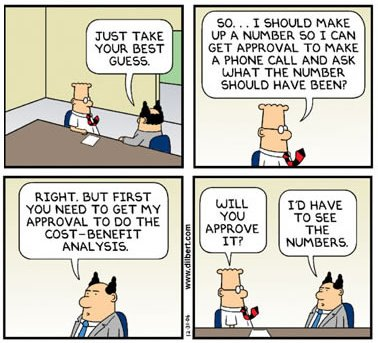
\includegraphics[width=\textwidth]{figures/dilbert-cost}
    \end{column}
  \end{columns}
\end{frame}

\end{document}
